\documentclass[a4paper,14pt]{extarticle}

\usepackage[utf8x]{inputenc}
\usepackage[T1]{fontenc}
\usepackage[russian]{babel}
\usepackage{hyperref}
\usepackage{indentfirst}
\usepackage{here}
\usepackage{array}
\usepackage{graphicx}
\usepackage{caption}
\usepackage{subcaption}
\usepackage{chngcntr}
\usepackage{amsmath}
\usepackage{amssymb}
\usepackage[left=2cm,right=2cm,top=2cm,bottom=2cm,bindingoffset=0cm]{geometry}
\usepackage{multicol}
\usepackage{multirow}
\usepackage{titlesec}
\usepackage{listings}
\usepackage{color}
\usepackage{enumitem}
\usepackage{cmap}
\usepackage{url}

\definecolor{green}{rgb}{0,0.6,0}
\definecolor{gray}{rgb}{0.5,0.5,0.5}
\definecolor{purple}{rgb}{0.58,0,0.82}

\lstdefinelanguage{none}{}

\lstset{
	language={none},
	inputpath={../logs/},
	backgroundcolor=\color{white},
	commentstyle=\color{green},
	keywordstyle=\color{blue},
	numberstyle=\color{gray}\scriptsize\ttfamily,
	stringstyle=\color{purple},
	basicstyle=\footnotesize\ttfamily,
	breakatwhitespace=false,
	breaklines=true,
	captionpos=b,
	keepspaces=true,
	numbers=left,
	numbersep=5pt,
	showspaces=false,
	showstringspaces=false,
	showtabs=false,
	tabsize=4,
	frame=single,
	morekeywords={},
	deletekeywords={},
	extendedchars=false,
	columns=fullflexible,
	literate=%
		{~}{{\raise.25ex\hbox{$\mathtt{\sim}$}}}{1}%
		{-}{-}{1}
}

\titleformat*{\section}{\large\bfseries} 
\titleformat*{\subsection}{\normalsize\bfseries} 
\titleformat*{\subsubsection}{\normalsize\bfseries} 
\titleformat*{\paragraph}{\normalsize\bfseries} 
\titleformat*{\subparagraph}{\normalsize\bfseries} 

\counterwithin{figure}{section}
\counterwithin{equation}{section}
\counterwithin{table}{section}
\newcommand{\sign}[1][5cm]{\makebox[#1]{\hrulefill}}
\newcommand{\equipollence}{\quad\Leftrightarrow\quad}
\newcommand{\no}[1]{\overline{#1}}
\graphicspath{{../pics/}}
\captionsetup{justification=centering,margin=1cm}
\def\arraystretch{1.3}
\setlength\parindent{5ex}
\titlelabel{\thetitle.\quad}

\setitemize{topsep=0em, itemsep=0em}
\setenumerate{topsep=0em, itemsep=0em}

\begin{document}

\begin{titlepage}
\begin{center}
	Санкт-Петербургский Политехнический Университет Петра Великого\\[0.3cm]
	Институт компьютерных наук и технологий \\[0.3cm]
	Кафедра компьютерных систем и программных технологий\\[4cm]
	
	\textbf{ОТЧЕТ}\\ 
	\textbf{по лабораторной работе}\\[0.5cm]
	\textbf{<<Data Mining>>}\\[0.1cm]
	Интеллектуальные системы\\[3.0cm]
\end{center}

\begin{flushright}
	\begin{minipage}{0.5\textwidth}
		\textbf{Работу выполнил студент}\\[3mm]
		гр. 3540901/91502 \hfill \sign[1.1cm] \hfill Дьячков В.В.\\[5mm]
		\textbf{Работу принял преподаватель}\\[5mm]
		\sign[2.1cm] \hfill к.т.н., доц. Бендерская Е.Н. \\[5mm]
	\end{minipage}
\end{flushright}

\vfill

\begin{center}
	Санкт-Петербург\\[0.3cm]
	\the\year
\end{center}
\end{titlepage}

\addtocounter{page}{1}

\tableofcontents
\newpage

\section{Программа работы}

\begin{enumerate}
	\item На примере одной из экспертных систем ExSys Corvid\footnote{\url{http://www.exsys.com/demomain.html}} укажите содержание компонентов:
	\begin{itemize}
		\item Диалоговый компонент
		\item База данных
		\item База знаний
		\item Решатель
	\end{itemize}
	\item Выполните лабораторные работы 1-6 из методических рекомендаций Д.И. Муромцев. Оболочка экспертных систем Exsys Corvid – СПб: СПб ГУ ИТМО, 2006. – 69 с.\footnote{\url{http://csd.faculty.ifmo.ru/dimour/ES/Corvid.pdf}}
	\item По приведенному описанию ЭС разработайте статическую экспертную систему для нахождения характерных неисправностей прибора Диск-250 ДД и метода их решения. Прибор показывающий и регистрирующий Диск-250 ДД предназначен для измерения и регистрации силы тока, а также неэлектрических величин, преобразованных в силу тока. Данная ЭС предназначена для использования слесарями в целях быстрого обнаружения неисправности и ее устранения. Привести в отчете:
	\begin{itemize}
		\item Перечень переменных с описанием их типа и значений;
		\item Дерево решений, разработанной Вами ЭС;
		\item Базу знаний, разработанной Вами ЭС;
		\item Интерфейс с пользователем (перечень вопросов, задаваемых пользователю).
	\end{itemize}
\end{enumerate}

\newpage

\section{Выполнение работы}

\subsection{Компоненты экспертной системы}

\begin{itemize}
	\item Диалоговый компонент
	\item База данных
	\item База знаний
	\item Решатель
\end{itemize}

\section{Лабораторные работы по CORVID}

\subsection{Создание простейшей системы}

В рамках данной работы создадим простейшую ЭС для принятия решения о замене лампочки в том случае, если она перегорела. На рис. \ref{fig:bulb_1} приведен логический блок разработанной ЭС.

\begin{figure}[H]
	\centering
	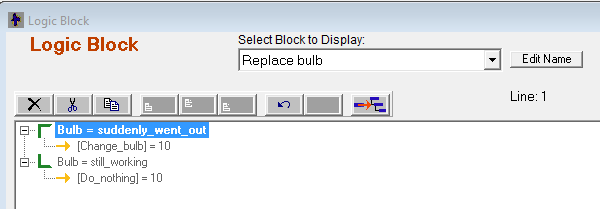
\includegraphics[width=\linewidth]{bulb_1}
	\caption{Логический блок ЭС}
	\label{fig:bulb_1}
\end{figure}

В листинге \ref{lst:bulb_1} приведен сгенерированный алгоритм работы ЭС.

\begin{lstlisting}[label=lst:bulb_1, caption={Алгоритм работы ЭС}]
IF:
	Bulb in your house suddenly went out
THEN:
	Change the bulb: Confidence = 10

IF:
	Bulb in your house still working
THEN:
	Do nothing: Confidence = 10
\end{lstlisting}

На рис. \ref{fig:bulb_2} приведен пользовательский интерфейс ЭС.

\begin{figure}[H]
	\centering
	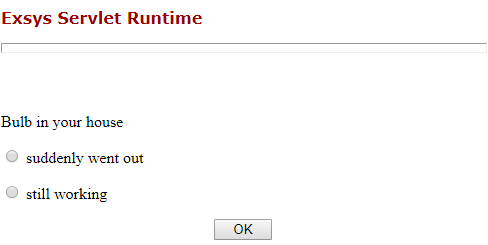
\includegraphics[width=0.7\linewidth]{bulb_2}
	\caption{Пользовательский интерфейс ЭС}
	\label{fig:bulb_2}
\end{figure}

На рис. \ref{fig:bulb_3} приведены результаты работы ЭС.

\begin{figure}[H]
	\centering
	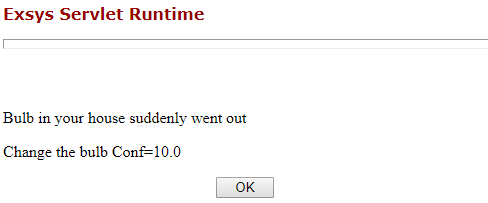
\includegraphics[width=0.7\linewidth]{bulb_3}
	\caption{Результаты работы ЭС}
	\label{fig:bulb_3}
\end{figure}

Таким образом, в рамках работы изучен интерфейс Exsys CORVID на примере простейшей экспертной системы.

\subsection{Улучшение интерфейса пользователя}

В рамках данной работы рассмотрим возможности форматирования интерфейса в системе Exsys CORVID.

На рис. \ref{fig:bulb_4} приведено изображение обновленного окна результатов. Был изменен шрифт и оставлено отображение только текстового значения.

\begin{figure}[H]
	\centering
	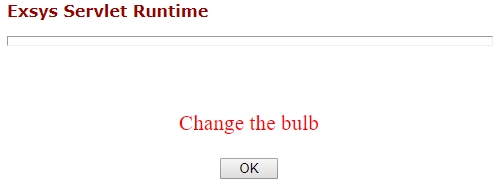
\includegraphics[width=0.7\linewidth]{bulb_4}
	\caption{Результаты работы ЭС}
	\label{fig:bulb_4}
\end{figure}

Заменить отображение вопроса на изображение не удалось по известным только разработчикам Exsys CORVID причинам.

\subsection{Усиление логики системы}

В рамках данной работы усовершенствуем логический блок имеющийся ЭС.


\begin{lstlisting}[label=lst:bulb_1, caption={Алгоритм работы ЭС}]
IF:
	Bulb in your house suddenly went out
AND:
	The other light in the room stay on
THEN:
	Change the bulb: Confidence = 10

\end{lstlisting}

\subsection{Обратная связь}

\subsection{Числовые переменные и [[]] подстановки}

\subsection{Переменные коллекции}

\section{Разработка статической ЭС}

\subsection{Переменные}

\subsection{Дерево решений ЭС}

\subsection{База знаний ЭС}

\subsection{Пользовательский интерфейс}

\newpage

\bibliographystyle{plain}
\addcontentsline{toc}{section}{Список литературы}
\bibliography{refs}

\end{document}
